\documentclass[aspectratio=169,11pt]{beamer}

\usetheme{Boadilla}
\usecolortheme{seahorse}
\useinnertheme{rectangles}
\useoutertheme{infolines}
\setbeamercolor{structure}{fg=blue!55!black}
\setbeamercolor{title}{fg=white,bg=blue!55!black}
\setbeamercolor{frametitle}{fg=blue!55!black}
\setbeamercolor{block title}{bg=blue!12,fg=blue!55!black}
\setbeamercolor{block body}{bg=blue!4}
\setbeamertemplate{navigation symbols}{}
\setbeamerfont{frametitle}{series=\bfseries,size=\large}
\setbeamerfont{title}{series=\bfseries,size=\Large}

\usepackage[T1]{fontenc}
\usepackage[utf8]{inputenc}
\DeclareFontShape{T1}{cmss}{b}{n}{<->ssub*cmss/bx/n}{}
\usepackage{amsmath,amssymb,bm}
\usepackage{graphicx}
\usepackage{tikz}
\usetikzlibrary{arrows.meta,positioning}

% ---------------- Macros ----------------
\newcommand{\uu}{\bm{u}}
\newcommand{\x}{\bm{x}}
\newcommand{\pp}{p}
\newcommand{\Rey}{\mathrm{Re}}
\newcommand{\avg}[1]{\overline{#1}}
\newcommand{\up}{\uu'}
\newcommand{\ubar}{\avg{\uu}}

\title[RANS I: Continuity]{RANS Part 1: Reynolds Decomposition \& the Mass Continuity Equation}
\author[Miller]{Laura A. Miller}
\institute[UArizona]{Department of Mathematics, University of Arizona}
\date{}

% Uncomment if you want speaker notes:
% \usepackage{pgfpages}
% \setbeameroption{show notes on second screen=right}

\begin{document}

% ---------------- Title ----------------
\begin{frame}
  \titlepage
  \vspace{-1.4em}
  \centering{\scriptsize Adapted from a \href{https://www.youtube.com/watch?v=mDt-HJEXK6g}{lecture by Steven L. Brunton}.}
  \\[2pt]{\tiny\color{black!55}AI tools were used to assist with formatting, organization, and clarification of the instructor's original notes.}
  \note{
  Goal today: set up time averaging + Reynolds decomposition, then apply it to incompressibility.
  End result: both mean flow and fluctuations are divergence-free.
  }
\end{frame}

% ---------------- Roadmap ----------------
\begin{frame}{Roadmap (Part 1)}
\begin{itemize}
  \item Start with incompressible Navier--Stokes (nondimensional form).
  \item Define the Reynolds decomposition: $\uu(\x,t)=\ubar(\x)+\up(\x,t)$ for a stationary mean.
  \item Define the time-average operator and its key properties.
  \item Plug decomposition into \textbf{mass continuity} $\nabla\cdot\uu=0$.
  \item Time-average to derive:
  \[
    \nabla\cdot\ubar = 0,
    \qquad
    \nabla\cdot\up = 0.
  \]
\end{itemize}
\note{
Keep this as a promise: we will not touch momentum closure today.
}
\end{frame}

% ---------------- Governing equations ----------------
\begin{frame}{Incompressible Navier--Stokes (nondimensional)}
We work with the incompressible Navier--Stokes equations:
\begin{align*}
\frac{\partial \uu}{\partial t} + (\uu\cdot\nabla)\uu &= -\nabla \pp + \frac{1}{\Rey}\,\Delta \uu,\\
\nabla\cdot\uu &= 0.
\end{align*}

\begin{itemize}
  \item $\uu(\x,t)\in\mathbb{R}^3$ is the velocity field.
  \item $\pp(\x,t)$ is pressure (scaled).
  \item $\Rey$ is the Reynolds number (the ratio of inertial to viscous effects for the chosen scales).
\end{itemize}

\textbf{Interpretation:} first line is  \textbf{momentum conservation}, second line is \textbf{mass conservation} (incompressibility).
\end{frame}

% ---------------- Vector components ----------------
\begin{frame}{Reminder: $\uu$ is a 3-component field}
Write
\[
\uu(\x,t) =
\begin{bmatrix}
u(\x,t)\\
v(\x,t)\\
w(\x,t)
\end{bmatrix},
\qquad
\x=(x,y,z).
\]

Then incompressibility is
\[
\nabla\cdot\uu = \frac{\partial u}{\partial x} + \frac{\partial v}{\partial y} + \frac{\partial w}{\partial z} = 0.
\]

\textbf{Today:} we will apply Reynolds averaging to this equation.
\end{frame}

% ---------------- Reynolds decomposition ----------------
\begin{frame}{Reynolds decomposition}
We decompose the flow into a mean and a fluctuation:
\[
\uu(\x,t) = \ubar(\x) + \up(\x,t).
\]

Component-wise:
\[
u = \avg{u} + u',\quad
v = \avg{v} + v',\quad
w = \avg{w} + w'.
\]

\begin{itemize}
  \item Mean flow $\ubar(\x)$ is \textbf{time-averaged}; it depends only on space under the stationarity assumption used here.
  \item Fluctuations $\up(\x,t)$ capture all remaining unsteady turbulent content.
\end{itemize}

\note{
Emphasize: in this setup, bar is time average; primes are deviations from that mean.
}
\end{frame}

% ---------------- Time average definition ----------------
\begin{frame}{Time average (stationary assumption)}
For a statistically stationary flow, define the long-time average at each spatial point:
\[
\avg{\uu}(\x) \;:=\; \lim_{T\to\infty}\frac{1}{T}\int_0^T \uu(\x,t)\,dt.
\]

\begin{itemize}
  \item We assume the relevant statistics are \textbf{stationary} and the long-time average is well defined.
  \item Then the fluctuation is defined by
  \[
  \up(\x,t) := \uu(\x,t) - \ubar(\x).
  \]
\end{itemize}

\textbf{Historical motivation:} point measurements (e.g., hot-wire anemometry) produce long time series at fixed $\x$. For nonstationary flows, an ensemble or finite-window average may retain time dependence.

\note{
Stationarity means statistics don’t change in time (after transients).
}
\end{frame}

\begin{frame}{A signal, its mean, and its fluctuation}
\centering
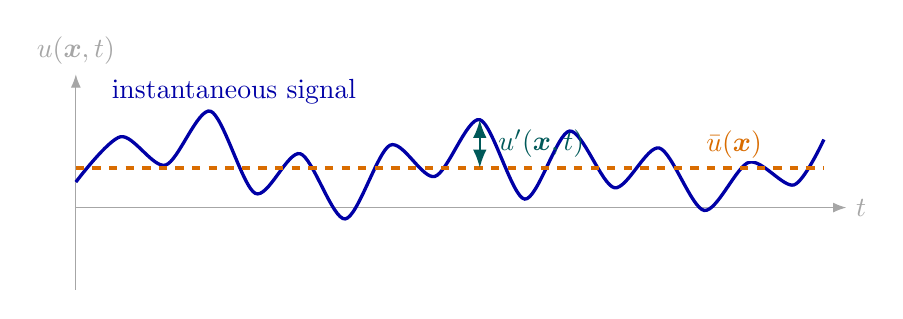
\begin{tikzpicture}[x=0.95cm,y=0.72cm,>=Latex]
  \draw[->,gray!70] (0,0) -- (10.3,0) node[right] {$t$};
  \draw[->,gray!70] (0,-1.45) -- (0,2.35) node[above] {$u(\x,t)$};
  \draw[blue!65!black,very thick,smooth]
    plot coordinates {(0,0.45) (0.6,1.25) (1.2,0.75) (1.8,1.70) (2.4,0.25)
    (3.0,0.95) (3.6,-0.20) (4.2,1.10) (4.8,0.55) (5.4,1.55)
    (6.0,0.15) (6.6,1.35) (7.2,0.35) (7.8,1.05) (8.4,-0.05)
    (9.0,0.80) (9.6,0.40) (10.0,1.20)};
  \draw[orange!85!black,dashed,very thick] (0,0.70) -- (10,0.70)
    node[pos=0.88,above=2pt,fill=white,inner sep=1pt] {$\bar u(\x)$};
  \draw[<->,teal!70!black,thick] (5.4,0.70) -- (5.4,1.55)
    node[midway,right=3pt] {$u'(\x,t)$};
  \node[blue!65!black,anchor=west] at (0.35,2.05) {instantaneous signal};
\end{tikzpicture}

\begin{block}{Pointwise identity}
At every sampled time, $u(\x,t)=\bar u(\x)+u'(\x,t)$, while $\overline{u'}=0$ by construction.
\end{block}
\end{frame}

\begin{frame}{Reynolds decomposition: illustration}
\centering
\includegraphics[width=0.55\textwidth]{pictures/5-2/Reynolds-decomposition.png}
\vfill
  \hfill {\footnotesize Source: McDonough, James (2009). Lectures in elementary fluid dynamics: physics, mathematics and applications.}
\end{frame}

\begin{frame}{Turbulent pipe flow}
\centering
\includegraphics[width=0.7\textwidth]{pictures/5-2/pipe-flow-turbulent.jpg}
\vfill
  \hfill {\footnotesize Source: https://www.tec-science.com/mechanics/gases-and-liquids/pressure-loss-in-pipe-systems/}
  \end{frame}
% ---------------- Why do this? ----------------
\begin{frame}{Why average? (model reduction viewpoint)}
Direct simulation of fully turbulent Navier--Stokes may require resolving:
\begin{itemize}
  \item largest energetic scales \textbf{and} smallest dissipative scales,
  \item often $\Rightarrow$ millions to billions of degrees of freedom.
\end{itemize}
\vfill

In many applications, we care about \textbf{mean quantities} (e.g., drag, lift, separation)
and perhaps a few low-order statistics of fluctuations.
\vfill

\begin{block}{Key idea}
Try to model $\ubar(\x)$ and selected statistics of $\up$ without resolving every eddy.
\end{block}

\end{frame}

% ---------------- Properties of averaging ----------------
\begin{frame}{Algebra you need: properties of time averages}
Let $\avg{\cdot}$ denote time averaging.

\begin{itemize}
  \item \textbf{Zero-mean fluctuation:} $\avg{\up}=0$ (by definition).
  \item \textbf{Linearity:} $\avg{u+v}=\avg{u}+\avg{v}$.
  \item \textbf{Idempotent:} $\avg{\avg{u}}=\avg{u}$.
  \item \textbf{Commutes with differentiation:}
  $\displaystyle\avg{\frac{\partial a}{\partial t}}=\frac{\partial \avg{a}}{\partial t}$
  (and likewise for spatial derivatives).
  \item \textbf{Mean of mean times quantity:} 
  $\avg{\avg{u}\cdot v}=\avg{u}\cdot \avg{v}$.
  \item \textbf{Mean times mean:} if $u=\avg{u}$ and $v=\avg{v}$ then $\avg{u\cdot v} = u \cdot v$.
\end{itemize}
\vfill

\begin{block}{Important warning (closure starts here)}
In general,
\[
\avg{u \cdot v}\neq \avg{u}\, \cdot \avg{v}.
\]
\end{block}


\end{frame}

% ---------------- Commuting derivatives ----------------
\begin{frame}{Commuting the average with spatial derivatives}
Because we average in \textbf{time} (not space), we typically use:
\[
\avg{\frac{\partial u}{\partial s}}
=
\frac{\partial}{\partial s}\avg{u},
\]
provided we can interchange differentiation and integration (regularity assumptions).

\begin{itemize}
  \item If we time average a derivative, it's the same as the derivative of the time average.
  \item This is what makes the continuity derivation clean.
  \item Note we are \textbf{not} averaging in space here.
\end{itemize}

\end{frame}

\begin{frame}{Variance and higher moments of the fluctuation}
\begin{block}{Important warning}
\[
\avg{u'^2}\neq 0
\]
\end{block}
\vfill
\begin{itemize}
  \item The time average of the fluctuation is zero, $\avg{\up}=0$.
  \item Its variance and higher-order moments generally are not zero.
  \item These higher moments are important in the dynamics of the fluid, and we will need to keep track of them.
  \item $R_{ij}=\avg{u'_i u'_j}$ has units of velocity squared. The dimensional turbulent-stress contribution is conventionally $-\rho R_{ij}$.
\end{itemize}
    
\end{frame}

\begin{frame}{The heart of the closure problem}
    \begin{itemize}
        \item We are trying to take this very complicated equation that varies in space and time and obtain the mean flow and selected fluctuation statistics.
        \item But we don't want to solve NS in space and time everywhere.
        \item This challenge is at the heart of the closure problem. We end up with more unknowns than equations.
        \item We will need to make approximations and assumptions based on physical intuition to build closure models to determine the unknowns.
        \item Data-driven and machine-learning models can assist with these approximations, but they must still respect the governing physics and be tested a posteriori.
    \end{itemize}
\end{frame}

% ---------------- Plug into continuity ----------------
\begin{frame}{Step 1: plug decomposition into continuity}
Start with incompressibility:
\[
\nabla\cdot\uu = 0.
\]

Substitute $\uu=\ubar+\up$:
\[
\nabla\cdot(\ubar+\up)=0
\quad\Rightarrow\quad
\nabla\cdot\ubar + \nabla\cdot\up = 0.
\]

In components:
\begin{align*}
\frac{\partial \avg{u}}{\partial x} + \frac{\partial \avg{v}}{\partial y} + \frac{\partial \avg{w}}{\partial z}
\;+\;
\frac{\partial u'}{\partial x} + \frac{\partial v'}{\partial y} + \frac{\partial w'}{\partial z}
=0.
\end{align*}

\note{
Point out: this identity holds pointwise in space and time.
}
\end{frame}

% ---------------- Time average the continuity equation ----------------
\begin{frame}{Step 2: time-average the continuity equation}
We can learn a lot by time averaging this equation, so take the time average of
\[
\nabla\cdot\ubar + \nabla\cdot\up = 0.
\]

Using commutation with spatial derivatives and $\avg{\up}=0$:
\[
\avg{\nabla\cdot\ubar} + \avg{\nabla\cdot\up} = 0
\quad\Rightarrow\quad
\nabla\cdot\ubar + \nabla\cdot\avg{\up}=0
\quad\Rightarrow\quad
\nabla\cdot\ubar = 0.
\]

\begin{block}{Result 1}
\[
\nabla\cdot\ubar = 0 \qquad\text{(mean flow is divergence-free).}
\]
\end{block}

\note{
Emphasize: this is a clean consequence of linearity + commutation + zero-mean prime.
}
\end{frame}

% ---------------- Deduce fluctuating divergence-free ----------------
\begin{frame}{Step 3: deduce divergence-free fluctuations}
Recall the pointwise identity:
\[
\nabla\cdot\ubar + \nabla\cdot\up = 0 \quad\text{(for all $\x,t$)}.
\]

But we just proved $\nabla\cdot\ubar=0$ (for all $\x$), hence
\[
\nabla\cdot\up = -\,\nabla\cdot\ubar = 0.
\]

\begin{block}{Result 2}
\[
\nabla\cdot\up = 0 \qquad\text{(fluctuations are divergence-free).}
\]
\end{block}

\note{
This is a nice moment: one equation gives two constraints after decomposition + averaging.
}
\end{frame}

% ---------------- Interpretation ----------------
\begin{frame}{Interpretation: what did we gain?}
We started with one constraint:
\[
\nabla\cdot\uu = 0.
\]

After Reynolds decomposition + time averaging we obtain:
\[
\nabla\cdot\ubar = 0,
\qquad
\nabla\cdot\up = 0.
\]

\begin{itemize}
  \item This will simplify bookkeeping in the momentum derivation.
  \item The hard part is \textbf{not} continuity---it’s what averaging does to \textbf{nonlinear products}.
\end{itemize}


\end{frame}

% ---------------- Preview of next lecture ----------------
\begin{frame}{Preview: momentum equation and closure}
Next, we will substitute
\[
\uu=\ubar+\up,\qquad \pp=\avg{\pp}+\pp'
\]
into
\[
\frac{\partial \uu}{\partial t} + (\uu\cdot\nabla)\uu = -\nabla \pp + \frac{1}{\Rey}\Delta\uu
\]
and time-average.

\end{frame}

% ---------------- End slide ----------------
\begin{frame}{Takeaways}
\begin{itemize}
  \item Reynolds decomposition: $\uu=\ubar+\up$ with $\avg{\up}=0$.
  \item Time averaging (stationary assumption) + commutation with spatial derivatives.
  \item Applying to continuity yields:
  \[
  \nabla\cdot\ubar=0,\qquad \nabla\cdot\up=0.
  \]
  \item Next: momentum averaging $\Rightarrow$ Reynolds stresses and the closure problem.
\end{itemize}
\end{frame}

\begin{frame}{References and scope}
\small
\begin{itemize}
  \item O. Reynolds, ``On the dynamical theory of incompressible viscous fluids and the determination of the criterion,'' \emph{Philosophical Transactions of the Royal Society A}, 186 (1895).
  \item S. B. Pope, \emph{Turbulent Flows}, Cambridge University Press (2000), Chapters 3--4.
  \item S. L. Brunton, lecture on Reynolds-averaged Navier--Stokes equations (linked on the title slide).
  \item J. M. McDonough, \emph{Lectures in Elementary Fluid Dynamics} (2009), source for the decomposition graphic.
\end{itemize}

\begin{block}{Scope of this derivation}
The deck uses a long-time average for a statistically stationary, incompressible, constant-property flow. Ensemble- or phase-averaged formulations use the same Reynolds rules when the chosen operator is linear and commutes with the required derivatives.
\end{block}
\end{frame}

\end{document}
